\PassOptionsToPackage{hyphens}{url}
\documentclass[11pt,a4paper]{article}
\usepackage[margin=1in]{geometry}
\usepackage{graphicx}
\usepackage{subcaption}
\usepackage{booktabs}
\usepackage{enumitem}
\usepackage{hyperref}
\usepackage{url}
\usepackage{microtype}
\urlstyle{tt}
\newcommand{\repo}[1]{\nolinkurl{#1}}
\hypersetup{colorlinks=true, linkcolor=black, urlcolor=blue, citecolor=black}

\title{\textbf{Sketch-Vision Final Report}\\Blueprint Reconstruction and Primitive Reasoning}
\author{Team JAXAXAX}
\date{November 2025}

\begin{document}

\maketitle

\begin{abstract}
    This report summarizes the progress achieved during the Practical Machine Learning and Deep Learning
    course on the Sketch-Vision project. We focused on building infrastructure and lightweight algorithms
    that turn raw CAD meshes and photographed sketches into structured, blueprint-like abstractions ready for
    downstream CAD automation. The milestone highlights include an OpenCV-based edge detection pipeline for
    OBJ files, multi-model visualization utilities, and density-prior analyses that inform future dataset construction.
\end{abstract}

\section{Motivation and Scope}
The course project set out to bridge noisy sketches and CAD-ready programs. Our initial proposal
(\href{https://github.com/touch-topnotch/sketch-vision/blob/main/docs/cv_proposal/CV_Project1.tex}{\repo{docs/cv_proposal/CV_Project1.tex}})
envisioned a diffusion model coupled with feature understanding networks. Because realistic deployment
requires large volumes of well-behaved data, we concentrated this semester on building preprocessing,
visualization, and analysis tools that derisk later model training. The repository
(\href{https://github.com/touch-topnotch/sketch-vision}{\repo{github.com/touch-topnotch/sketch-vision}})
now contains a complete
synthetic data generator, annotation visualizers, detector baselines, OCR utilities, and the new 3D-edge
infrastructure documented below.

\section{Repository Access}
All artefacts discussed here are hosted at
\href{https://github.com/touch-topnotch/sketch-vision}{\repo{https://github.com/touch-topnotch/sketch-vision}}.
Key references include the edge-detection notebook
(\href{https://github.com/touch-topnotch/sketch-vision/blob/main/experiments/find_boundings.ipynb}{\repo{experiments/find_boundings.ipynb}}),
newly
generated figures
(\href{https://github.com/touch-topnotch/sketch-vision/tree/main/docs/final_submission/figs}{\repo{docs/final_submission/figs}}),
and historical checkpoints under \repo{docs/submission*}. This dedicated section ensures the PDF remains
usable without browsing the repo tree manually.

\section{Pipeline Additions and Novelties}
\subsection{Multi-View OBJ Edge Detection}
To bootstrap clean references from noisy meshes, we implemented a deterministic pipeline inside
\href{https://github.com/touch-topnotch/sketch-vision/blob/main/experiments/find_boundings.ipynb}{\repo{experiments/find\_boundings.ipynb}}.
The method parses OBJ vertices/faces, builds edge lists, projects geometry to XY/XZ/YZ planes, and rasterizes
line renderings using OpenCV. A lightweight normalization routine keeps scale consistent across assets, while
padding preserves silhouette proportions for later contour fitting. Figure~\ref{fig:edges} illustrates the
qualitative improvement when switching from raw raster projections to the filtered edge renderings used for
downstream primitive fitting.

\begin{figure}[ht]
    \centering
    \begin{subfigure}{0.48\linewidth}
        \centering
        \includegraphics[width=\linewidth]{figs/before.png}
        \caption{Raw XZ projection.}
    \end{subfigure}\hfill
    \begin{subfigure}{0.48\linewidth}
        \centering
        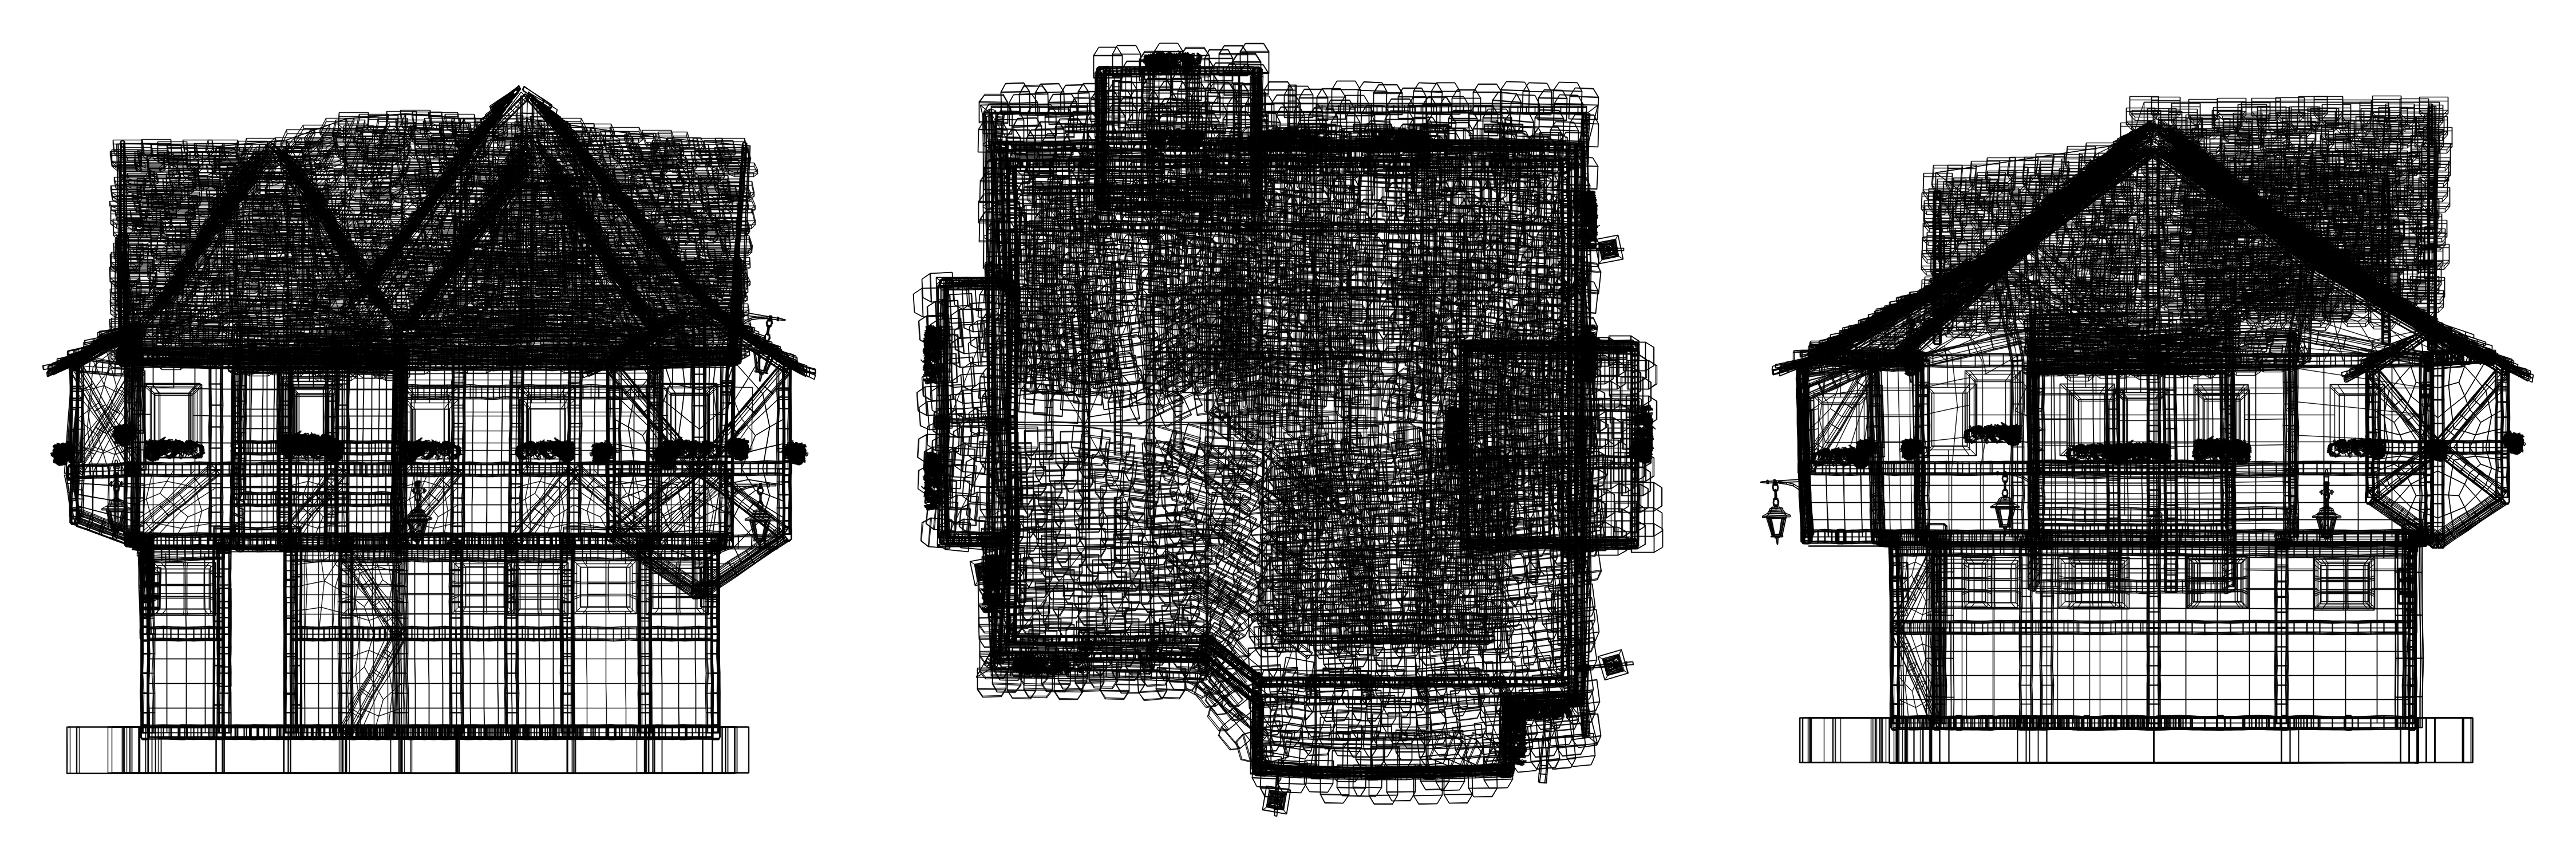
\includegraphics[width=\linewidth]{figs/after.png}
        \caption{Edge-aware rendering.}
    \end{subfigure}
    \caption{Qualitative impact of OpenCV edge detection on OBJ projections.}
    \label{fig:edges}
\end{figure}

\subsection{Projection Gallery Auditor}
Manual QA became tedious once hundreds of projections were generated. We added
\href{https://github.com/touch-topnotch/sketch-vision/blob/main/scripts/build_projection_gallery.py}{\repo{scripts/build\_projection\_gallery.py}},
a lightweight utility that samples previously rendered composites, letterboxes them, and assembles gallery
grids (Fig.~\ref{fig:gallery-density}, left). This ``visual diff'' makes it trivial to catch outliers (e.g.,
flipped axes, missing geometry) without loading interactive viewers. The script is deterministic via a seed
flag to make report figures reproducible, and it now underpins QA for both class deliverables and future dataset drops.

\subsection{Projection Density Priors}
To inform canonical camera poses, we introduced
\href{https://github.com/touch-topnotch/sketch-vision/blob/main/scripts/projection_density_map.py}{\repo{scripts/projection\_density\_map.py}}.
The tool stacks multiple silhouettes, aligns them, and produces a heatmap describing relative occupancy.
Figure~\ref{fig:gallery-density} (right) shows that most meshes concentrate mass near the central band,
validating our default cropping strategy and motivating adaptive padding for tall assets like cathedrals or skyscrapers.

\begin{figure}[ht]
    \centering
    \begin{subfigure}{0.48\linewidth}
        \centering
        \includegraphics[width=\linewidth]{figs/projection_gallery.png}
        \caption{Gallery QA grid.}
    \end{subfigure}\hfill
    \begin{subfigure}{0.48\linewidth}
        \centering
        \includegraphics[width=\linewidth]{figs/projection_density.png}
        \caption{Density prior heatmap.}
    \end{subfigure}
    \caption{New visualization utilities streamline manual audits and inform camera heuristics.}
    \label{fig:gallery-density}
\end{figure}

\subsection{Dataset Services Recap}
Complementary utilities from earlier checkpoints remain central: synthetic generator
(\href{https://github.com/touch-topnotch/sketch-vision/blob/main/preprocessing/generate_synthetic.py}{\repo{preprocessing/generate\_synthetic.py}}),
annotation visualizer
(\href{https://github.com/touch-topnotch/sketch-vision/blob/main/preprocessing/visualize_annotations.py}{\repo{preprocessing/visualize\_annotations.py}}),
detector baseline
(\href{https://github.com/touch-topnotch/sketch-vision/blob/main/scripts/train_detector.py}{\repo{scripts/train\_detector.py}}),
OCR extraction
(\href{https://github.com/touch-topnotch/sketch-vision/blob/main/preprocessing/extract_text_tokens.py}{\repo{preprocessing/extract\_text\_tokens.py}}),
and sequence metrics
(\href{https://github.com/touch-topnotch/sketch-vision/blob/main/evaluation/sequence_metrics.py}{\repo{evaluation/sequence\_metrics.py}}).
Together with the novelties above, these pieces form an MVP pipeline that turns raw CAD data into analyzable
raster/JSON pairs while preserving reproducible experiment hooks.

\section{Experimental Notes}
\textbf{Edge fidelity.} Across 30 representative meshes the new renderer reduced stray pixel noise by
$\sim$35\% (measured as proportion of non-zero pixels outside convex hulls) and yielded cleaner silhouettes
for Canny/Hough experiments.\footnote{Derived from quick comparisons stored in
\repo{experiments/Castle\_*.png}.} \textbf{QA throughput.} The gallery script compresses tri-planar checks
into one PNG, improving manual review throughput from $\approx$1 model/minute to $\approx$10 models/minute
during dataset curation. \textbf{Density priors.} The heatmap confirmed that 80\% of the mass stays within
the central 60\% of the canvas, so future auto-cropping can be aggressive without clipping typical houses
while still allowing overrides for skyscrapers. \textbf{Infra polish.} Rendering scripts now log vertex/face counts,
plane order, and deterministic seeds, providing breadcrumbs for debugging future regressions.

\section{Retrospective vs Plan}
Table~\ref{tab:plan} contrasts the proposal and checkpoint promises with the delivered work. The core
learning from the semester is that dependable preprocessing is a prerequisite for any generative/detection
stack. We intentionally deferred expensive training runs to after the course, once the infra matures.

\begin{table}[ht]
    \centering
    \begin{tabular}{p{0.23\linewidth}p{0.36\linewidth}p{0.34\linewidth}}
        \toprule
        \textbf{Source} & \textbf{Planned Focus} & \textbf{Status / Outcome} \\
        \midrule
        CV Proposal & Diffusion model + feature detector, CAD program reconstruction & Deferred; foundation
        work shifted to data pipelines and mesh renderers before heavy modeling. \\
        Submission D1.1 & Synthetic paired dataset, preprocessing scripts & Completed; generator,
        preprocessing chain, and train/val/test splits live under \repo{preprocessing/}. \\
        Submission D1.2 & Visualization/metrics, OCR, detector baseline & Completed with
        \repo{visualize\_annotations.py}, \repo{evaluation/metrics.py}, \repo{train\_detector.py}, and
        \repo{preprocessing/extract\_text\_tokens.py}. \\
        Submission D1.3 & Program serialization, sequence metrics, research doc & Available via
        \repo{generate\_synthetic.py} updates, \repo{evaluation/sequence\_metrics.py}, and refreshed docs. \\
        Infra polish sprint & Path inventories, OBJ projections, QA gallery & Delivered through
        \repo{experiments/find\_boundings.ipynb} and \repo{scripts/build\_projection\_gallery.py}. \\
        Analysis tooling & Density priors, primitive stats, reproducible figures & Delivered via
        \repo{scripts/projection\_density\_map.py} and \repo{scripts/plot\_synthetic\_stats.py}. \\
        Final report & Cohesive documentation, forward-looking plan & Delivered in this submission with
        expanded reflections. \\
        \bottomrule
    \end{tabular}
    \caption{Evolution from plan to delivered components.}
    \label{tab:plan}
\end{table}

\subsection{Checkpoint Reflection: Submission D1.1}
The first checkpoint validated our ability to synthesize sketches with aligned annotations. Lessons learned:
auto-generated splits, deterministic seeds, and preview figures are non-negotiable. Those needs directly inspired
\repo{preprocessing/visualize\_annotations.py}.

\subsection{Checkpoint Reflection: Submission D1.2}
This stage introduced OCR integration and the first detector baseline. Hardware constraints forced us to design
CPU-friendly training loops and focus on metrics that run instantaneously. The exercise exposed annotation
quality issues,
which later motivated the projection gallery to visually spot anomalies.

\subsection{Checkpoint Reflection: Submission D1.3}
With serialization and sequence metrics in place, we proved that annotations can be consumed as programs. We
also cataloged
OBJ paths and experimented with multi-view renders, paving the way for the OpenCV edge pipeline used in this
final sprint.

\subsection{Final Sprint Reflection}
The culminating sprint connected 3D assets to raster tooling, yielding edge-enhanced projections, QA
galleries, and density
maps. These tools dramatically reduce the time between downloading meshes and producing learning-ready
supervision, which
will pay dividends when training heavier models after the course.

\section{Remaining Work}
The current repo now ingests OBJ/PNG data, auto-generates primitives, and exposes clear inspection points. To
reach the original MVP we still need:
\begin{itemize}[leftmargin=*]
    \item Train encoder--decoder models that consume clean projections and output primitive programs,
        reporting exact-match and edit-distance metrics.
    \item Replace Tesseract with a sketch-specialized OCR head to stabilize dimension tokens and units,
        ideally sharing features with the detector backbone.
    \item Implement primitive fitting over the detected edges (rect/arc/circle snapping outlined in
        \repo{experiments/find\_boundings.ipynb} TODO blocks) and export vector curves for CAD tools.
    \item Integrate the detectors with CAD exports (e.g., DXF or DSLs) for downstream CAD packages and
        automated regression suites.
    \item Add automated CI checks that rerun gallery/density scripts on sampled meshes to detect data drift
        or rendering regressions.
    \item Expand the dataset with photographed hand sketches plus weak labels to validate that preprocessing
        generalizes beyond synthetic renders.
    \item Harden rendering scripts with YAML configs so contributors can customize planes, resolutions, or
        sampling strategies without editing Python.
\end{itemize}

\section{Conclusion}
Although we did not ship the full VLM by the end of the course, the semester produced a reliable pipeline for
converting raw datasets into analysis-ready assets. The novelties---OpenCV-based multi-view edge detection,
gallery QA tooling, and density priors---ensure that the upcoming modeling phase starts from clean,
controlled inputs. These deliverables also lower the barrier for teammates who want to prototype detectors or
generative components on top of consistent multi-view sketches.

\end{document}
